\chapter{Estado del arte}
\bigskip

Los principios básicos de los algoritmos genéticos fueron establecidos por Holland (1975), y se encuentran bien descritos en varios textos a lo largo de los años, como los estudios de Goldberg (1989), Davis (1991), Michalewicz (1992) o Reeves (1993), afianzando los conceptos y permitiendo trabajar sobre una buena base a futuros investigadores.

\bigskip
Son muchos y muy variados los ámbitos en los que se usan los algoritmos genéticos. Sirven para crear componentes automovilísticos, analizar expresiones de genes o hasta desarrollar aprendizajes de comportamiento para robots, por ejemplo. Incluso se usan en aquellos que otros métodos no consiguen resolver o tiene problemas, o dichos métodos se pueden llegar a conjuntar con los algoritmos genéticos para así mejorarlos.

\bigskip
Aunque no se garantiza que el algoritmo genético encuentre la solución óptima del problema, éste encontrará soluciones de un nivel aceptable, en un tiempo competitivo con el resto de los algoritmos de optimización combinatoria. 

\bigskip
Esto hace que se estudie y se intente mejorar y optimizar dichos algoritmos, siendo un campo con mucha transcendencia en la actualidad.

\bigskip
Constan de varias partes, como la selección de candidatos, operadores de cruce, funciones de evaluación y optimización o mutación. En este trabajo nos centraremos en la parte de optimización, donde se evalúan los individuos generados y que serán posibles soluciones al problema. Existen multitud de funciones de optimización, pero nos centraremos en 2: Ackley y Rastrigin.

\bigskip
La función de Ackley se publicó por primera vez en ``A connectionist machine for genetic hillclimbing`` por David H. Ackley en 1987 y se extendió a la dimensión arbitraria en ``Evolutionary algorithms in theory and practice: evolution strategies, evolutionary programming, genetic algorithms`` por Thomas Bäck en 1996.

\bigskip
\begin{figure}[h]
	\centering
	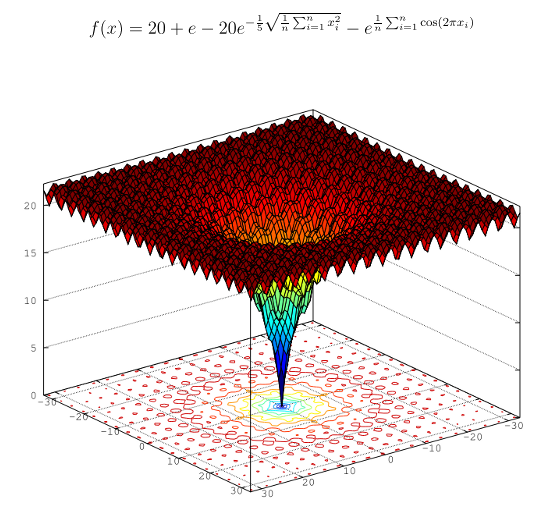
\includegraphics[width=0.7\linewidth]{../images/ackley}
	\caption[Función y representación de la función de optimización de Ackley]{Función y representación de la función de optimización de Ackley}
	\label{fig:ackley}
\end{figure}


\bigskip
Años antes, en 1974, Rastringin en "Systems of extremal control" propone otra función de optimización, para ser generalizada en 1991 por Mühlenbein.

\bigskip
\begin{figure}[h]
	\centering
	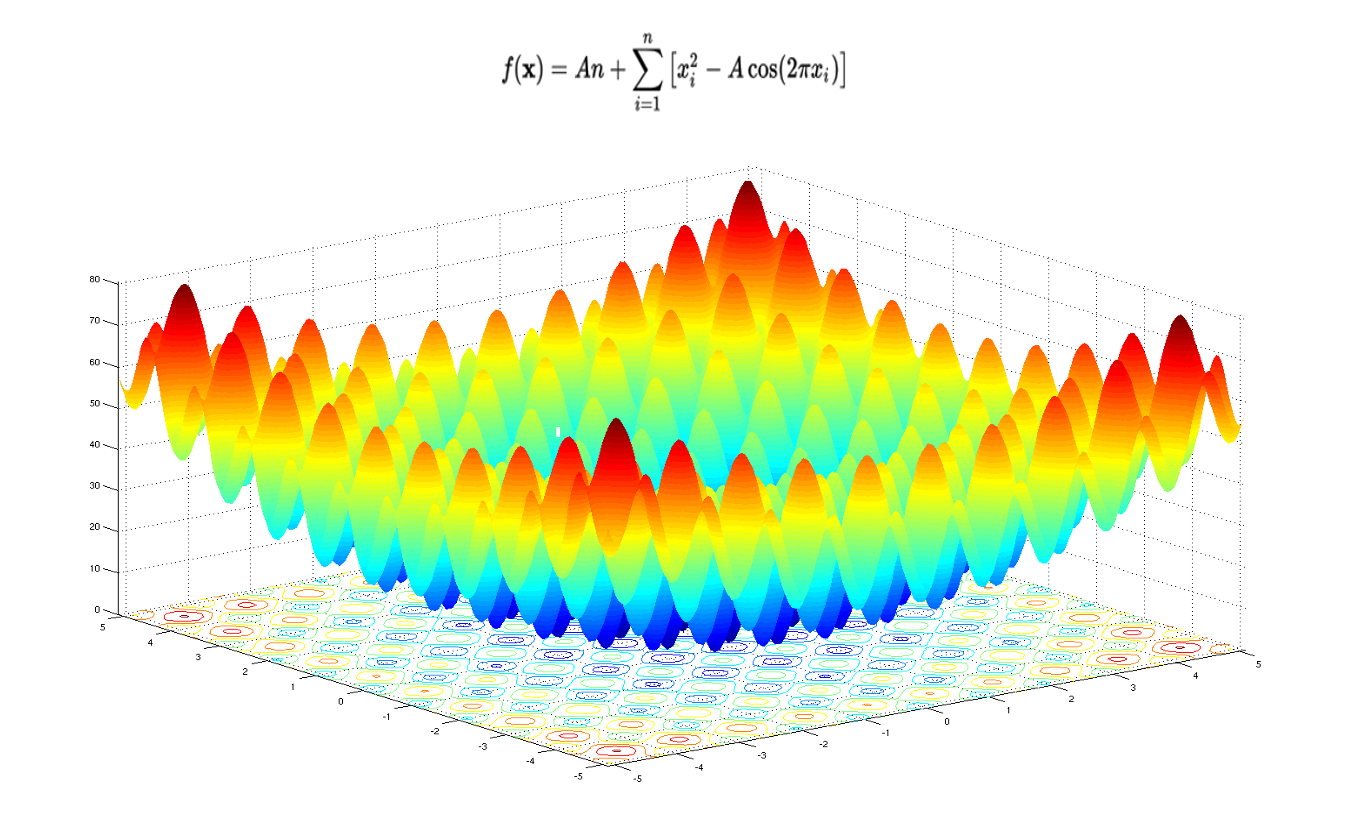
\includegraphics[width=0.7\linewidth]{../images/rastrigin}
	\caption[Función y representación de la función de optimización de Rastrigin]{Función y representación de la función de optimización de Rastrigin}
	\label{fig:rastrigin}
\end{figure}

\bigskip
Este trabajo se centrará en estas 2 funciones de optimización, ofreciendo un algoritmo genético que pueda ser optimizado mediante Ackley o Rastrigin.



\newpage
\section{Actualidad}
\bigskip

En la actualidad la mayoría de los usuarios que necesitan procesar un algoritmo genético lo hacen ellos mismos, con programas adaptados de terceros o desarrollados por ellos mismos. Esto conlleva un trabajo extra de estudio, implementación y corrección de dichos programas. 

Podemos encontrar algunos programas \cite{agpython} \cite{agjava} \cite{agmatlab} para ser ejecutados por el cliente, o servicios web que realizan algoritmos genéticos donde la mayoría son ejemplos o demostraciones de algoritmos genéticos y sus soluciones \cite{agandar} \cite{agcoche}.


Pero ninguno usa la computación paralela aprovechando la potencia de las GPUs. Viendo que hay disponible en el ámbito de dicha paralelización vemos que hay grandes empresas que han lanzado lenguajes de programación enfocados a aprovechar el procesamiento mediante la GPU: CUDA \cite{nvidiacuda}, AMD OpenCL APP \cite{paralelizacionamd}, BrookGPU \cite{brookgpu}, PeakStream \cite{peackstream} o RapidMind \cite{rapidmind}:

\begin{itemize}
	\item CUDA: arquitectura de cálculo paralelo de NVIDIA. Se basa en el lenguaje C y C++, por lo que, junto con la cantidad de dispositivos de la marca, existe una gran comunidad y documentación.
	
	\item AMD OpenCL™ Accelerated Parallel Processing: herramienta de AMD que permite el cómputo mediante GPUs. Se basa en los lenguajes OpenCL y C++, por lo que se pueden usar para acelarar aplicaciones.
	
	\item BrookGPU: programa (en versión \textit{beta}) de la Universidad de Stanford para aprovechar la paralelización en tarjetas gráficas AMD y NVIDIA. Para trabajar con el se usa una extensión de ANSI C.
	
	\item PeakStream era un programa para paralelizar el procesamiento con grandes rendimientos en tarjetas AMD, comprado por Google en 2007 \cite{peackstreamcomprada}, y tras esto, a dejado de ofrecer mantenimiento.
	
	\item RapidMind, que tambíen se basa en C++, es comprada por Intel en 2009 y pasa a ser Intel Array Building Blocks \cite{rapidmindcomprada}, pero sigue estando en forma experimental. 
	
\end{itemize}

Tras ver las distintas opciones, con sus distintas ventajas e inconvenientes, se decide centrar en CUDA. Es un proyecto activo, tiene numerosas actualizaciones, cuenta con mucha comunidad para resolver dudas y fomentar su desarrollo, y tiene numerosas facilidades, como un SDK \cite{nvidiadeveloper} y varias herramientas para sus desarrolladores. Por todo esto se escoge CUDA para desarrollar el trabajo.

\bigskip
CUDA surgió en 2006, cuando NVIDIA lanzó por primera vez al mercado una GPU capaz de renderizar gráficos en 3D y que incluyó la posibilidad de ejecutar, usando CUDA, programas escritos en lenguaje C.

\bigskip
\begin{figure}[h]
	\centering
	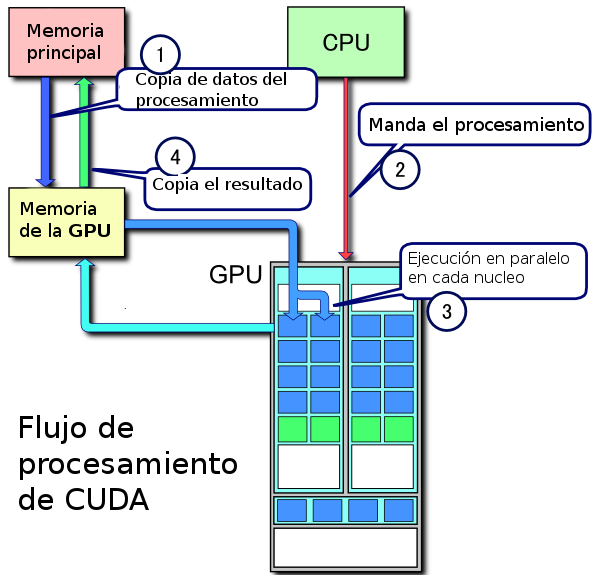
\includegraphics[width=0.6\linewidth]{../images/flujocuda}
	\caption[Ejemplo de flujo de procesamiento  CUDA]{Ejemplo de flujo de procesamiento CUDA}
	\label{fig:flujocuda}
\end{figure}


Gracias a su eficiencia energética y gran potencia, desde entonces NVIDIA ofrece la capacidad de sus tarjetas gráficas para grandes centros de datos y otras instituciones tanto científicas como gubernamentales, permitiendo dibujar gráficos y ejecutar diversos programas aprovechando.

Incluso se utilizan versiones reducidas para potenciar las aplicaciones tanto de teléfonos móviles, ordenadores portátiles y tablets, entre
otros.


\bigskip
En este campo hay algunos proveedores, como Impact  \cite{cudaimpact} o gpuOcelot \cite{cudagpuocelot} que ofrecen herramientas para la computación de algoritmos estándar o del código que genere el usuario, pero  realizando el cómputo desde las GPUs de los clientes, y nunca enfocados específicamente a resolver algoritmos genéticos.

\bigskip
Otras opciones permiten ejecutar CUDA en servidores externos, pero se necesita enviar una solicitud de uso y adaptarse a sus restricciones y capacidad, como en rCUDA \cite{rcuda}
o desplegar toda una instancia en un IaaS y desarrollar dentro: Amazon Web Services \cite{amazoncuda}.

\bigskip
Con esto se puede ver que podemos encontrar servicios que realicen algoritmos genéticos, o servicios que usen CUDA, pero no hay servicios que combinen ambos.


\bigskip
\section{Clientes}
\bigskip

¿Que usuarios necesitan computar algoritmos genéticos?

Por ejemplo, cualquier estudiante que quiera comprobar los distintos resultados del algoritmo genético cambiando sus parámetros. También el personal de investigación trabaja con multitud de algoritmo genéticos, y con grandes consumos de recursos. Junto con la potencia de cómputo y la accesibilidad que proporcionaremos simplificaríamos el trabajo de dicho personal. 

Además el servicio será accesible a cualquier usuario, y con su interfaz sencilla e intuitiva dichos usuarios no necesitarán una preparación especial para usarlo. 

\bigskip
\section{Competidores}
\bigskip

Como se cita antes, existen ejemplos o plantillas de algoritmos genéticos \cite{agpython} \cite{agjava} \cite{agmatlab} que los usuarios pueden usar, pero necesitan para su uso un trabajo extra para su instalación, desarrollo o ajustes. Además de este trabajo extra, se ven limitados por las capacidades de sus dispositivos, pues los algoritmos se tendrán que lanzar en local.

Para evitar dichas limitaciones, podemos usar la paralelización de los algoritmos, pero los trabajos que encontramos se encuentran en una versión de CUDA obsoleta \cite{paralelizacioncuda} (y simplemente exponiendo el código) o son estudios del servicio sin llegar a ser implementado \cite{optimizacionparalelizacioncuda}. Se busca entonces un servicio que ofrezca computación desde un servidor externo. Se pueden ver servicios que computan directamente CUDA \cite{rcuda} u ofrecen instancias con acceso a GPUs \cite{amazoncuda}  pero nunca especializados en algoritmos genéticos.


\bigskip
\section{Conclusiones}
\bigskip

Si se busca un servicio de computación externo (que ofrezca una mayor potencia de computación usando GPUs) de algoritmos genéticos no llegamos a encontrar nada que cumpla con nuestro requisitos: o son servicios en local para lanzar algoritmos genéticos o son servicios externos que nos ofrecen computación aprovechando la paralelización de CUDA, pero sin llegar a ofrecer ninguna aproximación de un algoritmo genético.

Viendo esto se encuentra una demanda que podemos cubrir con nuestro servicio, motivando a su análisis y desarrollo.







